\part{Computational Graph Level}


    \section{ROS Master}
        The ROS Master provides name registration and lookup to the rest of the Computation Graph.
        It acts as a nameservice, storing topics and services registration information for nodes. Nodes communicate with the Master to report 
        their registration information.
        As these nodes communicate with the Master, they can receive information about other registered nodes and make connections as appropriate.
        Nodes connect to other nodes directly; the Master only provides lookup information.
        Nodes communication is established over the TCPROS protocol, which uses standard TCP/IP sockets.
        There is always only one master in the network, nodes must know network address of which.


    \section{Nodes}
        Nodes are basic processes that perform computation, written through ROS client library (roscpp, rospy). Each node has its own name 
        (graph resource name) that identify it and a node type (package resource name).
        They are combined into a graph and communicate with each other using:
        \begin{itemize}
            \item topics
            \item services
            \item actions
        \end{itemize}
        Furthermore, they have variables which can be managed using:
        \begin{itemize}
            \item parameter server
            \item dynamic reconfigures
        \end{itemize}    


        \subsection{Python node}
        
            \begin{enumerate}
                \item Package structure
\begin{minted}[bgcolor=LightGray, fontsize=\footnotesize, baselinestretch=1.2]{shell}
/pkg_name
    /nodes
        node.py
    CMakeLists.txt
    package.xml
\end{minted}
            \item Make the node executable
\begin{minted}[bgcolor=LightGray, fontsize=\footnotesize, baselinestretch=1.2]{shell}
chmod +x node.py
\end{minted}

            \end{enumerate}


        \subsection{C++ node}
            \begin{enumerate}
                \item Package structure
\begin{minted}[bgcolor=LightGray, fontsize=\footnotesize, baselinestretch=1.2]{shell}
/pkg_name
    /src
        node.cpp
    /include
        node.h
    CMakeLists.txt
    package.xml
\end{minted}
            \item Make the node executable
\begin{minted}[bgcolor=LightGray, fontsize=\footnotesize, baselinestretch=1.2]{shell}
include_directories(
  include 
  ${catkin_INCLUDE_DIRS}
)
add_excutable(node src/node.cpp)
\end{minted}

            \end{enumerate}





    \section{Communication}


        \begin{tabular}[c]{ |p{2.5cm}||c|p{4cm}|p{3cm}|p{2cm}| }
            \hline
            Messages & Structure  & Application & Example & Tools \\
            \hline
            \hline
            Topics & .msg & one-way continuous data stream & sensors data & rostopic \\
            \hline
            Services & .srv & blocking task for processing a request & trigger, request state, computations & rosservice \\
            \hline
            Actions & .action & non-blocking preemptable goal-oriented tasks & navigation, grasping, motion & actionlib \\
            \hline
            Parameter Server & .param & global constant parameters & names, settings, calibration data, robot setup & rosparam \\
            \hline
            Dynamic reconfigure & .cfg & local, tunable parameters & controller parameters & ?? \\
            \hline
        \end{tabular}


        \subsection{Topics}
            Topics are named buses for unidirectional, streaming communication between nodes, in which there are:
            \begin{itemize}
                \item Publisher – nodes that send data
                \item Subscriber – nodes interested in data
            \end{itemize}
            The master initializes the topic communication and tracks all the information.
            Topics’ default protocol is TCPROS (TCP/IP-based). Another protocol is UDPROS (UDP-based) only for roscpp, that is a low-latency, lossy transport, so is best suited for tasks like teleoperation.
            \\
            Rules:
            \begin{itemize}
                \item Any node can publish a message to any topic
                \item Any node can subscribe to any topic 
                \item Any node can both publish and subscribe to any topics at the same time
                \item Multiple nodes can publish and subscribe to the same topic
            \end{itemize}



        \subsection{Services}
            Services are a pair of messages exchanged between nodes:
            \begin{itemize}
                \item Client (Response) – node providing a service
                \item Server (Request) – node requesting a service which gives back the response
            \end{itemize}
            Rules:
            \begin{itemize}
                \item Any node can implement services (server)
                \item Any node can call services (client)
                \item Servers call are synchronous/blocking
            \end{itemize}



        \subsection{Actions}
            Actions, like services, are messages exchanged between two nodes, providing additional features:
            \begin{itemize}
                \item ActionClient – node providing a task and the possibility to cancel that task
                \item ActionServer – node receiving a task which give back the status, the result and the feedback
            \end{itemize}
            The used protocol is the “ROS Action Protocol” which is built on top of ROS messages (High-level).
            
            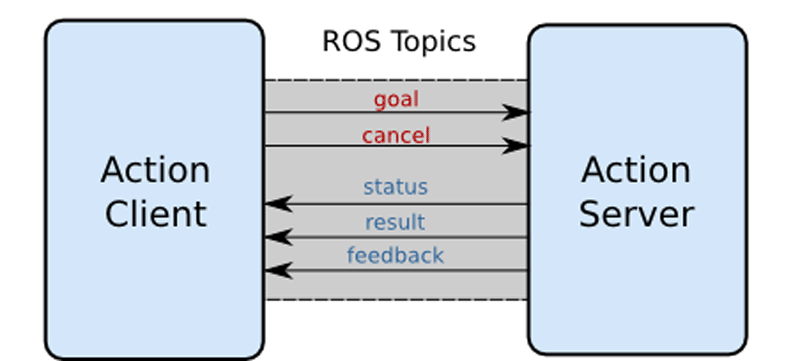
\includegraphics[width=16cm]{pictures/comm_actions.png}
            
            Rules:
            \begin{itemize}
                \item Goal - can be messages, services or parameters data structures used to send goals
                \item Cancel – used to send cancel requests
                \item Status – used to notify clients on the current state of every goal in the system
                \item Feedback - provides information about the incremental progress of a goal
                \item Result - send upon completion of the goal
            \end{itemize}



        \subsection{Parameter Server}
            A parameter server is a shared, multi-variate dictionary implemented using XMLRPC. Nodes can use this server to store and retrieve parameters runtime, for static, non-binary data.
            Supported types:
            \begin{itemize}
                \item strings
                \item 32-bit integers
                \item doubles
                \item float
                \item booleans
                \item lists of elements
                \item dictionary
                \item base64-encoded binary data
                \item iso8601 dates
            \end{itemize}

        
        
        \subsection{Dynamic reconfigure}
            The dynamic reconfigure is a package providing a means to update parameters at runtime without having to restart the node.

            CMakeLists.txt
\begin{minted}[bgcolor=LightGray, fontsize=\footnotesize, baselinestretch=1.2]{xml}
generate_dynamic_reconfigure_options(
    cfg/dynamic.cfg
)
\end{minted}

%             ## CMakeLists.txt
% ```
% # Dynamic reconfigure
% generate_dynamic_reconfigure_options(
%   cfg/dynamic.cfg
% )
% ```
        






    \section{Bags}
        It’s a format for saving, storing and playback ROS message data in .bag files.
        Bag files can be played back in ROS to the same topic they were recorded from, or even remapped to new topics.

    

    \section{Launch files}




        

